\section{Overview of NLP}
Natural Language Processing (NLP) is a field at the intersection of linguistics, computer science, and artificial intelligence. It enables machines to understand, interpret, and generate human language.

\subsection{Key Applications}
\begin{itemize}
    \item Automatic Summarisation
    \item Information Extraction
    \item Machine Translation
    \item Question Answering
    \item Text Classification
\end{itemize}

\section{Challenges in NLP}
\begin{itemize}
    \item \textbf{Syntax:} Structure of a sentence.
    \item \textbf{Semantics:} Meaning of words and sentences.
\end{itemize}

\section{Approaches in NLP}
\subsection{Rule-Based}
\begin{itemize}
    \item Hand-coded rules based on expert knowledge.
    \item Easy to interpret and debug.
    \item Does not require large volumes of data.
\end{itemize}

\subsection{Data-Driven}
\begin{itemize}
    \item Infers rules from data.
    \item Accuracy improves with more data.
    \item May be biased or hard to interpret.
    \item More flexible and scalable.
\end{itemize}

\section{Probabilistic Models}
\subsection{Markov Chains}
Used in both rule-based and data-driven systems depending on how transition probabilities are derived (e.g., n-gram frequency).

\subsection{Bayes' Rule}
\[
P(B|A) = \frac{P(A|B) \cdot P(B)}{P(A)}
\]

\subsection{Naive Bayes Classifier}
Assumes independence among features to compute the probability of a class given the features.

\section{Formal Grammars}
\subsection{Context-Free Grammar (CFG)}
Abstracts meaning from text to represent structure. It uses production rules to define possible sentence structures.

\subsection{Syntax Tree Example}

\begin{center}
\Tree [.S [.NP [.D She ] ] [.VP [.V saw ] [.NP [.D the ] [.N city ] ] ] ]
\end{center}

\section{Word Representation}
\subsection{Tokenisation}

\begin{itemize}
    \item \textbf{Character-level:} Good for spell-checking, compact
    \item \textbf{Word-level:} Intuitive, but memory-intensive
    \item \textbf{Subword-level:} Balanced approach, most commonly used
\end{itemize}

\subsection{One-Hot Encoding}
Represents words as binary vectors.

\subsection{Word2Vec}
Learns vector representations (embeddings) of words based on their context.

\subsubsection{Continuous Bag of Words (CBOW)}
Predicts target word from context.

\begin{tcolorbox}[title=CBOW Architecture]
\begin{itemize}
    \item \textbf{Input:} One-hot encoded vectors of context words
    \item \textbf{Hidden Layer:} Trains word embeddings
    \item \textbf{Output:} Softmax over vocabulary
\end{itemize}
\end{tcolorbox}

\section{Neural Networks in NLP}
\subsection{Perceptron}
A basic unit in neural networks:
\[
y = \begin{cases}
1 & \text{if } w \cdot x + b > 0 \\
0 & \text{otherwise}
\end{cases}
\]

\subsection{Feedforward Neural Network}
\begin{center}
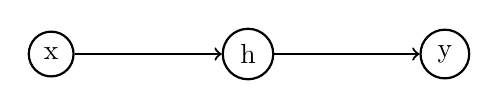
\begin{tikzpicture}[->, thick, node distance=2.5cm]
  \node[circle, draw] (1) {x};
  \node[circle, draw, right of=1] (2) {h};
  \node[circle, draw, right of=2] (3) {y};
  \draw[->] (1) -- (2);
  \draw[->] (2) -- (3);
\end{tikzpicture}
\end{center}

\subsection{Encoder-Decoder Architecture}
Used for sequence-to-sequence tasks like translation.

\subsection{Recurrent Neural Networks (RNNs)}
Processes sequences step by step and maintains a hidden state.

\begin{itemize}
    \item Captures sequential dependencies.
    \item Suffers from vanishing gradients and depth issues.
\end{itemize}

\subsection{Attention Mechanism}
Weighs hidden states by importance.

\[
\text{Attention}(Q, K, V) = \text{softmax}\left( \frac{QK^T}{\sqrt{d_k}} \right)V
\]

\section{Transformers}

\subsection{Key Features}
\begin{itemize}
    \item Self-attention
    \item Parallel processing
    \item Positional encoding
\end{itemize}

\subsection{Architecture Diagram}
\begin{center}
\begin{tikzpicture}[node distance=1cm and 1.5cm, align=center, font=\small, >=Latex]

% Encoder
\node (input) [draw, rectangle] {Input Tokens};
\node (posenc) [draw, rectangle, below=of input] {Positional Encoding};
\node (selfatt) [draw, rectangle, below=of posenc] {Self-Attention (Multi-Headed)};
\node (encnet) [draw, rectangle, below=of selfatt] {Feedforward Neural Net};
\node (encout) [draw, rectangle, below=of encnet] {Encoded Representation};

% Decoder
\node (prevword) [draw, rectangle, right=3cm of input] {Previous Word};
\node (decpos) [draw, rectangle, below=of prevword] {Positional Encoding};
\node (decselfatt) [draw, rectangle, below=of decpos] {Masked Self-Attention};
\node (decattenc) [draw, rectangle, below=of decselfatt] {Attention over Encoder};
\node (decnet) [draw, rectangle, below=of decattenc] {Feedforward Neural Net};
\node (output) [draw, rectangle, below=of decnet] {Output Word};

% Arrows
\draw[->] (input) -- (posenc);
\draw[->] (posenc) -- (selfatt);
\draw[->] (selfatt) -- (encnet);
\draw[->] (encnet) -- (encout);

\draw[->] (prevword) -- (decpos);
\draw[->] (decpos) -- (decselfatt);
\draw[->] (decselfatt) -- (decattenc);
\draw[->] (decattenc) -- (decnet);
\draw[->] (decnet) -- (output);

\draw[->, dashed] (encout.east) -- ++(1,0) -- ++(0,-5.8) -- (decattenc.east);

\end{tikzpicture}
\end{center}

\subsection{Advantages}
\begin{itemize}
    \item Enables parallel training.
    \item Captures long-term dependencies.
\end{itemize}

\subsection{Limitations}
\begin{itemize}
    \item Memory intensive for long sequences.
\end{itemize}

\section{Exam Preparation Summary}
\begin{itemize}
    \item Activation Functions: Step, Sigmoid
    \item Perceptron = Linear function + Step
    \item NLP Language Models: N-grams, Neural, Transformers
\end{itemize}